% reset memory of all acronyms, so \ac will print out full name of acronym!
\acresetall 
\hyphenation{Bundes-anstalt} % because ngerman/babel doesn´t know it correctly... 
%TODO: need to fix hyphenation of "Bundesanstalt" in ac
\chapter{Einleitung}
\paragraph{Motivation der Arbeit}
irgendwas Orginelles...
\begin{figure}[H]
	\centering
	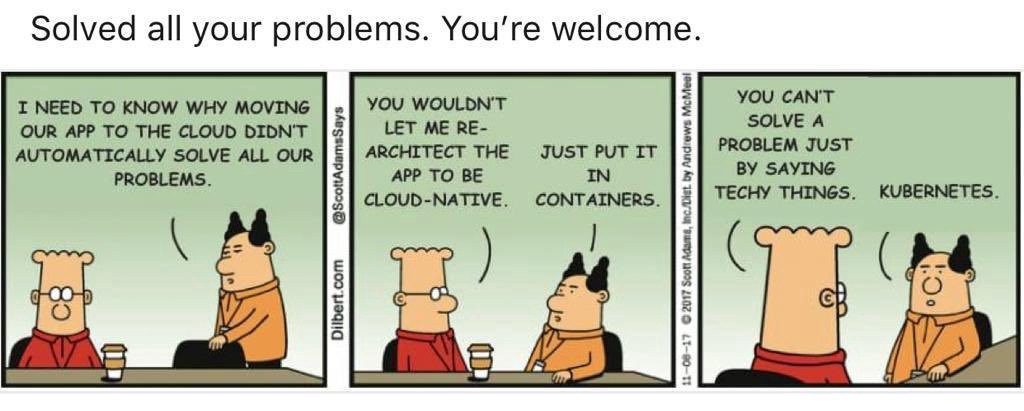
\includegraphics[scale=0.33]{img/dilbertCloud.jpeg}
	\caption{Dilbert Comic zu \textsc{Kubernetes}}
	{\footnotesize Quelle: \cite{DilbertKubernetes}\par}
	{\footnotesize Redaktionelle Anmerkung: Abbildung nur als komprimiertes Format verfügbar (Qualitätseinbuße)}
\end{figure}

\paragraph{Problemstellung/-abgrenzung}

\paragraph{Zielstellung der Arbeit}

\paragraph{Forschungsfragen/-design}
Die Forschungsfragen mit der sich diese Bachelorarbeit beschäftigen wird, sind eine direkte Konsequenz aus der Zielstellung und aus den unternehmensinternen Anforderungen an einen möglichen automatisierten Prozess. Dabei liegt der Fokus auf der Betrachtung beider Teildisziplinen der Wirtschaftsinformatik, nämlich der Informatik und der Wirtschaft -- jedoch wird der größere Teil dieser Arbeit einen informationstechnischen Fokus besitzen. Die folgende Aufzählung nennt die einzelnen Forschungsfragen, die im weiteren Verlauf ein gemeinsames Ergebnis erbringen werden. Dieses ist in Kapitel \vref{kritischeBetrachtung} zu finden.
\begin{enumerate}
	\item Wie können Container-Anwendungen den Prozess des automatisierten \enquote{Deployments\footnote{die Definition dieses Begriffes ist in Kapitel \vref{defDeployment} zu finden}} unterstützen?
	\item Welche wirtschaftlichen Vorteile hat der Einsatz von Container auf den Prozess des automatisierten \enquote{Deployments}?
	\item Welche besonderen sicherheitstechnischen Aspekte muss ein solcher Prozess im Bereich der Versicherung erfüllen?
\end{enumerate}
%TODO: Definition Technologie-Wertekette, Red Hat, OpenShift :Platzhalter <Defintion/>
Die Forschungsfrage eins wird einen Ist-Zustand analysieren. Dieser enthält eine Prozessanalyse, eine identifizierte Technologie-Wertekette\footnote{Definition: <Defintion/>} sowie einen Anforderungskatalog der Entwicklungsabteilungen an den zu konzeptionierenden \enquote{Deployment}-Prozess für die Container-Anwendungen. Danach wird ein Konzept eines container-basierten, automatisierten \enquote{Deployment}-Prozesses erstellt, dabei wird die Methodologie und das eigentliche Konzept erläutert. Die Forschungsfrage eins schließt mit einem Teilergebnis ab. \par
Die Forschungsfrage zwei beschäftigt sich mit den wirtschaftlichen Vorteilen eines Einsatzes der Container auf den Prozess des automatisierten \enquote{Deployment}-Prozesses. Dabei werden die Erstellung eines \enquote{Business Case\footnote{engl. Geschäftsszenario}}, die Prüfung der Übereinstimmung der Ziele dieser Arbeit mit der Geschäftsstrategie der \ac{SVI} und mögliche Disharmonien dieser identifiziert. Außerdem entsteht eine Konzeption eines verbesserten Geschäftsszenarios, das die Kosteneinsparpotentiale und die Zielharmonisierung enthalten wird. Ein Ausblick schließt die Forschungsfrage zwei ab. \par
Die Forschungsfrage drei identifiziert sicherheitsrelevante Anforderungen, die nicht nur die funktionalen/nicht-funktionalen Anforderungen einer Anwendung betreffen, sondern auch die komplette \ac{AWL}. Dabei beeinflusst die \ac{BaFin} und auch verschiedene \textsc{DIN/ISO}-Normen diese Anforderungen. Außerdem soll analysiert werden, wie bei der Beschaffung von \enquote{open source}- bzw. \enquote{closed source}-Anwendungen mögliche Schwachstellen identifiziert werden, die potentielle Angriffsvektoren in der \ac{AWL} eröffnen würden, und wie mit diesen verfahren wird. Dabei soll versucht werden Rückschlüsse auf die Anwendung \textsc{OpenShift\footnote{<Definition/>}} von \textsc{Red Hat\footnote{<Definition/>}} zu ziehen. Auch hier wird ein Teilergebnis diese Forschungsfrage abschließen


\paragraph{Einordnung der Abteilung in den Geschäftsprozess}
Die Abteilung \ac{IE2}, die sich im Bereich der Organisationseinheit \ac{IE} befindet, befasst sich in erster Linie mit dem Transport (\enquote{Deployment}) von Software-Artefakten der einzelnen Software-Produkte der \ac{SVI}. Diese werden für die \ac{SV} entwickelt, betrieben und gewartet. Zu den zentralen Aufgaben der Abteilung gehören die Planung, Durchführung und Überwachung der \enquote{Build/Deployment}-Prozesse auf den verschiedenen Serverumgebungen. Des weiteren stellt \ac{IE2} die Einspielung von datenbank-relevanten Objekten sicher. Auch entwickelt sie die Bau- und Transportprozesse kontinuierlich weiter und passt diese an die sich ständig veränderten Anforderung der Entwicklungsabteilungen an. Von zentraler Bedeutung ist die Planung und Durchführung der Veröffentlichungen der neuen Versionen einer zu betreuenden Anwendung. Zu dieser Aufgabe gehören auch Aufbau und Bereitstellung der Systemtest-, Releasetest- und Produktions-Umgebungen. Eine weitere zentrale Aufgabe, die nach der Organisationsumstrukturierung am 01.01.2020 in der Abteilung \ac{IE2} angesiedelt wurde, ist das Umgebungsmanagement. Die Aufgaben dieses Teilbereichs befasst sich mit folgenden Inhalten: Planung von Aktivitäten in der Produktionsumgebung, Planung und Koordination der Infrastruktur und Notfall-\enquote{Fixe} der Produktion, der allgemeinen \enquote{Patch}-Planung; Beratung zur Erweiterung, Koordination und Planung von verschiedenen Testumgebungen. Außerdem ist das Umgebungsmanagement Teil des \ac{CAB}, das ein Gremium nach der Sammlung \ac{ITIL} darstellt. Dieses ist für die Freigabe von \enquote{Changes} verantwortlich und hat ständige, wie auch der Situation angepasste, Mitglieder. 

\paragraph{Aufbau der Arbeit}
In Kapitel \vref{ff1} \par
In Kapitel \vref{ff2} \par
In Kapitel \vref{ff3} \par
In Kapitel \vref{kritischeBetrachtung}
